

\chapter{Appendice A}

\section{Proposta alternativa di Dataset delle Zone}
\label{nostraProposta}
Prima di approdare al dataset delle zone di cui abbiamo discusso nella Sez. \ref{zone}, abbiamo ipotizzato e implementato un metodo in grado di restituirci un dataset delle zone in cui suddividere l'Abruzzo prendendo come punto di partenza il dataset delle zone prodotto dall'esecuzione della seguente \textit{query} su PostGres:
\begin{quote}
CREATE TABLE \textit{GeoArea\_split8} (
\newline
\textit{id} serial PRIMARY KEY,
\newline
\textit{geom} geometry (Polygon, 3004))
\newline
\newline
INSERT INTO \textit{GeoArea\_split8} (geom) 
\newline
SELECT ST\_Subdivide(geom,8)
\newline
FROM \textit{Geo\_Area}
\end{quote}

L'invocazione della funzione \textbf{ST\_Subdivide()} sulla geometria che descrive \textit{GeoArea} genera $24142$ zone in cui è suddiviso il territorio abruzzese, di cui è possibile avere una visione d'insieme in Fig. \ref{nostrodataset}.
\begin{figure}[h]
\centering
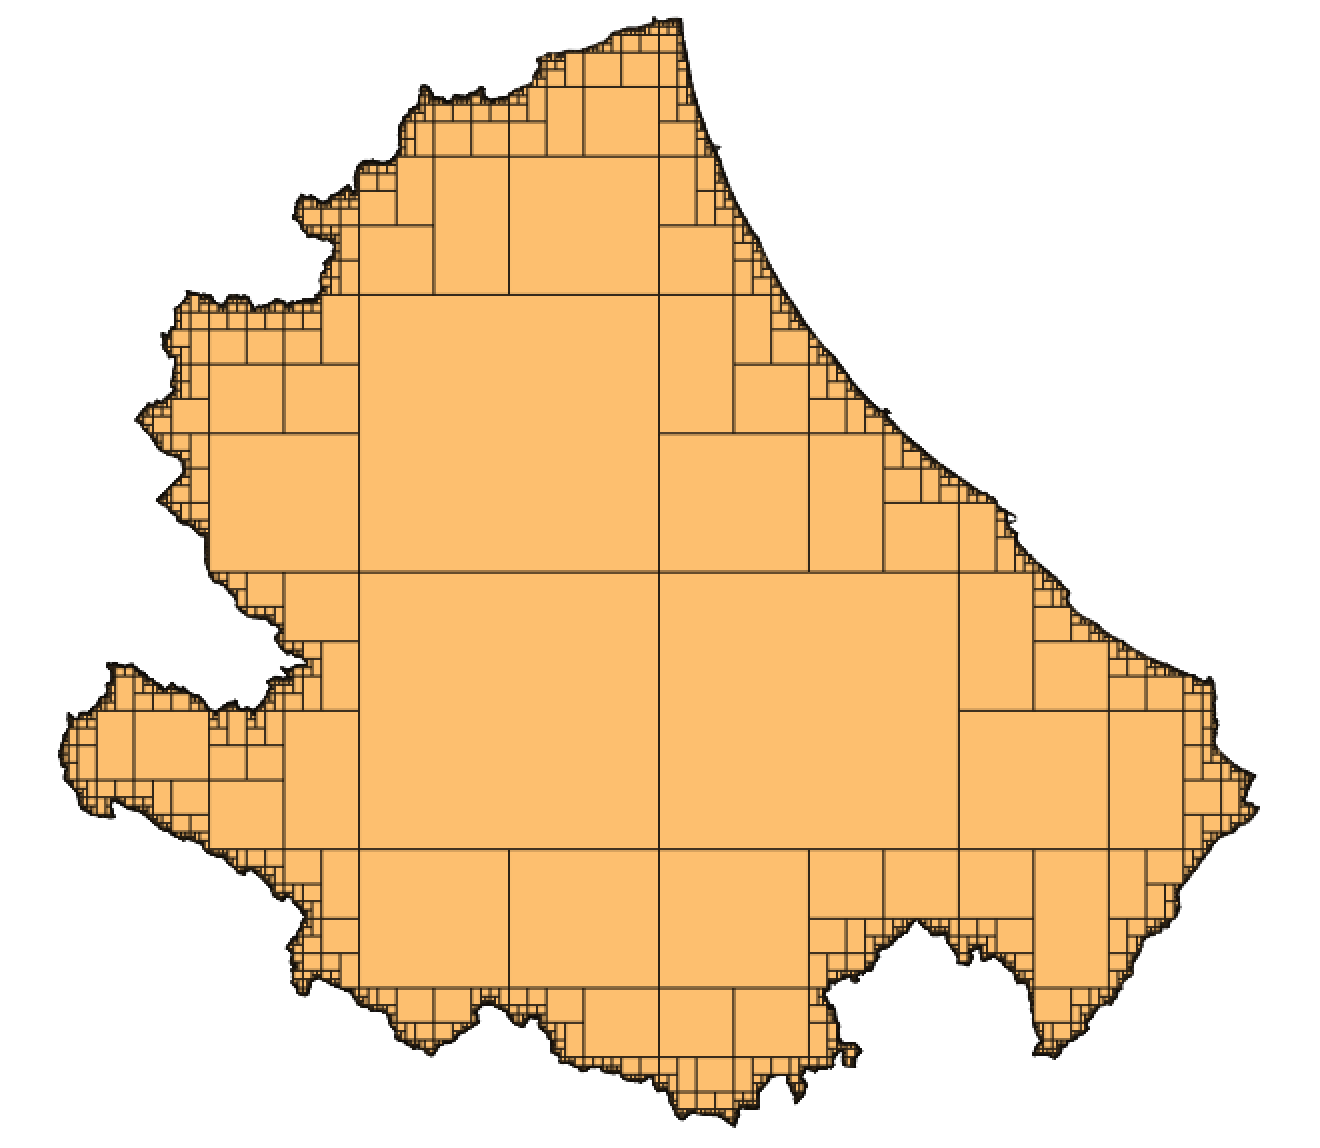
\includegraphics[width=0.4\textwidth]{img/nostrodataset}
\caption{Visione d'insieme delle $24142$ zone generate}
\label{nostrodataset}
\end{figure}
L'esame della Fig. \ref{bordo} fornisce una visione più nitida del tipo di suddivisione effettuata da ST\_Subdivide(). Esso in prossimità del \textit{boundary} della \textit{GeoArea} costruisce poligoni di forma irregolare aventi al massimo otto vertici, mentre tutte le altre aree sono dei quadrati di area crescente via via che ci si sposta verso il centro della \textit{GeoArea}.
Al fine di realizzare un'analisi quantitativa dell'esito del partizionamento della \textit{GeoArea} si riportano in tabella \ref{topMax} e in tabella \ref{topMin} rispettivamente le dieci aree con area maggiore e le dieci con aree minore.

\begin{table}[h]
\centering
\begin{tabular}{|c|c|}
\hline
\rowcolor{lightgray}
Area (kmq)                  & Perimetro (km)             \\
\hline
$3,46$ $\times$ $10^{-11}$  & $3,55$ $\times$ $10^{-5}$  \\
\hline
$1,14$ $\times$ $10^{-10}$  & $5,74$ $\times$ $10^{-5}$  \\
\hline
$3,11$ $\times$ $10^{-10}$  & $8,64$ $\times$ $10^{-5}$  \\
\hline
$3,21$ $\times$ $10^{-10}$  & $8,84$ $\times$ $10^{-5}$  \\
\hline
$6,29$ $\times$ $10^{-10}$  & $19,22$ $\times$ $10^{-5}$ \\
\hline
$6,46$ $\times$ $10^{-10}$  & $14,01$ $\times$ $10^{-5}$ \\
\hline
$6,86$ $\times$ $10^{-10}$  & $14,38$ $\times$ $10^{-5}$ \\
\hline
$8,90$ $\times$ $10^{-10}$  & $16,65$ $\times$ $10^{-5}$ \\
\hline
$11,81$ $\times$ $10^{-10}$ & $19,91$ $\times$ $10^{-5}$ \\
\hline
$13,05$ $\times$ $10^{-10}$ & $17,51$ $\times$ $10^{-5}$ \\
\hline
\end{tabular}
\caption{Top 10 aree più piccole}
\label{topMin}
\end{table}

\begin{table}[h]
\centering
\begin{tabular}{|c|c|}
\hline
\rowcolor{lightgray}
Area (kmq) & Perimetro (km) \\ \hline
$1231,2$   & $140,5$          \\ \hline
$1231,2$   & $140,5$         \\ \hline
$1231,2$   & $140,5$          \\ \hline
$307,8$    & $70,2$           \\ \hline
$307,8$    & $70,2$           \\ \hline
$307,8$    & $70,2$           \\ \hline
$307,8$    & $70,2$           \\ \hline
$307,8$    & $70,2$           \\ \hline
$307,8$    & $70,2$           \\ \hline
$307,8$    & $70,2$          \\ \hline
\end{tabular}
\caption{Top 10 aree più grandi}
\label{topMax}
\end{table}


Come si può vedere chiaramente i valori del perimetro e dell'area delle varie zone presentano davvero molti ordini di grandezza di differenza, ragion per cui è necessario un duplice approccio di elaborazione allo scopo di ottenere un dataset delle zone più omogeneo e tale per cui le varie zone abbiano un'estensione quantomeno paragonabile tra loro:
\begin{itemize}
\item Frazionamenti successivi dei poligoni interni "\textit{enormi}" ;
\item Accorpamenti successivi dei poligoni lungo il bordo.
\end{itemize}
\subsection{Processamento dei poligoni interni}
Al fine di realizzare un algoritmo in grado di realizzare dei frazionamenti successivi dei poligoni interni "enormi" presenti nel dataset delle zone che abbiamo preso come punto di partenza abbiamo realizzato uno studio della funzione \textbf{ST\_Subdivide()}, con lo scopo di comprendere quali sono i suoi limiti applicativi. Da questo studio è emerso che tale funzione risulta essere inapplicabile per $500$ delle $24142$ zone in cui abbiamo diviso il territorio, ciò ha determinato la creazione di questi poligoni interni "enormi". Questi $500$ elementi presentano un'area maggiore di $0,1$ kmq (valore che ci siamo prefissati come valore medio delle aree delle zone in cui dividere la \textit{GeoArea}) e hanno numero di vertici inferiore ad $8$, motivo per cui non sono processabili ulteriormente tramite la funzione ST\_Subdivide().\newline
Abbiamo ricercato dunque un'altra funzione che potesse venirci in aiuto per raggiungere il nostro obiettivo e consultando il manuale PostGIS 2.3.2dev abbiamo ritenuto opportuno utilizzare la funzione \textbf{ST\_Segmentize} per processare queste $500$ zone "\textit{problematiche}". Applicando tale funzione abbiamo ottenuto $37875$ zone la cui area massima è pari a $0,0005$ mq. E' stato necessario, di conseguenza, implementare un meccanismo di aggregazione di tali zone con lo scopo di ottenere zone con area media pari a $0,1$ kmq. Il metodo di aggregazione che abbiamo proposto e implementato sfrutta approccio \textit{random}: per ogni zona abbiamo utilizzato la funzione \textbf{ST\_buffer()} 
%specificare che raggio abbiamo utilizzato per la funzione st_buffer e il centro centroide? 
%inserire immagine che aiuta a comprendere 
per individuare le zone confinanti con essa, candidate ad essere aggregate con essa; Tramite la funzione \textbf{random} determino quali tra esse dovranno essere effettivamente aggregate con la zona in esame al fine di raggiungere l'obiettivo che ci siamo prefissati.
\subsection{Processamento dei poligoni lungo il bordo}
Come abbiamo già discusso nella Sez. \ref{nostraProposta} le zone presenti sul bordo hanno un'area distante molti ordini di grandezza rispetto l'obiettivo che ci siamo prefissati. Di conseguenza è stato necessario implementare un meccanismo di aggregazione di tali zone con lo scopo di ottenere delle aree con estensione più accettabile e vicina al valore medio che ci siamo posti come obiettivo: \newline
\begin{itemize}
\item Per ogni zona problematica del bordo, che andremo a chiamare $z_bordo$, andiamo a realizzare un buffer con un certo raggio (che a livello implementativo abbiamo fissato a 150m) con lo scopo di costruire un cerchio.
\item Tale cerchio verrà intersecato, tramite la funzione \textbf{ST\_Intersect()}, con tutte le zone problematiche del bordo al fine di individuare quali sono le zone che intersecano la sua geometria, che andremo a chiamare $z_cerchio$.
\item Per ogni $z_cerchio$, sfruttando la funzione \textbf{ST\_relate} e la definizione di \textit{DE-9IM matrix pattern}, riusciamo a stabilire se risulta essere adiacente con la zona $z_bordo$ (la funzione \textbf{ST\_relate} restituirà \textit{true} o \textit{false} se l'intersezione tra le due zone, rappresentate come poligoni, è una linea/geometria di dimensione 1).

\end{itemize}



